%%%%%%%%%%%%%%%%%%%%%%%%%%%%%%%%%%%%%%%%%%%%%%%%%%%%%%%%%%%
%% Master's Thesis of Jukka Pajarinen
%%%%%%%%%%%%%%%%%%%%%%%%%%%%%%%%%%%%%%%%%%%%%%%%%%%%%%%%%%%
\documentclass[finnish, authoryear]{config/tauthesis}
\usepackage{pgfplots}
\pgfplotsset{compat=1.15}
\usepackage{subcaption}
\usepackage{amsmath, amssymb, amsthm, bm}
\usepackage{float}
\usepackage{soul}
\newcommand{\verbcommand}[1]{\texttt{\textbackslash #1}}
\newtheorem{lause}{Lause}[chapter]
\newtheorem{theorem}[lause]{Theorem}
\newtheorem{apulause}[lause]{Apulause}
\newtheorem{lemma}[lause]{Lemma}
\theoremstyle{definition}
\newtheorem{maaritelma}{Määritelmä}[chapter]
\newtheorem{definition}[maaritelma]{Definition}
\loadglsentries[main]{tex/04_sanasto.tex}
\makeglossaries
\addbibresource{tex/00_zotero-referenssit.bib}

%%%%%%%%%%%%%%%%%%%%%%%%%%%%%%%%%%%%%%%%%%%%%%%%%%%%%%%%%%%
%% Front matter
%%%%%%%%%%%%%%%%%%%%%%%%%%%%%%%%%%%%%%%%%%%%%%%%%%%%%%%%%%%
\begin{document}
\frontmatter
\title
  {Web-käyttöliittymän hyväksymistestauksen priorisointi painotetun verkon avulla}
  {Web User Interface Acceptance Testing Prioritization with a Weighted Graph}
\subtitle{}{}
\author{Jukka Pajarinen}
\finishdate{2019}{12}{31}
\thesistype{Diplomityö}{Master's Thesis}
\facultyname
  {Informaatioteknologian ja viestinnän tiedekunta}
  {Faculty of Information Technology and Communication Sciences}
\programmename{Tietotekniikan DI-ohjelma}{Degree Programme in Information Technology}
\keywords
  {hyväksymistestaus, painotettu verkko, priorisointi, jatkuva integraatio, testiautomaatio}
  {acceptance testing, weighted graph, prioritization, continuous integration, test automation}
\maketitle
\abstract{tex/01_tiivistelma.tex}
\otherabstract{tex/02_abstract.tex}
\preface{tex/03_alkusanat.tex}{Tampereella}
\tableofcontents
\listoffigures
\listoftables
\glossary

%%%%%%%%%%%%%%%%%%%%%%%%%%%%%%%%%%%%%%%%%%%%%%%%%%%%%%%%%%%
%% Main matter
%%%%%%%%%%%%%%%%%%%%%%%%%%%%%%%%%%%%%%%%%%%%%%%%%%%%%%%%%%%
\mainmatter
\chapter{Johdanto} \label{ch:05_johdanto}
  Tämä mallipohja liittyy Tampereen yliopiston tekniikan alan opinnäytteiden kirjoitusohjeisiin \parencite{kirjoitusohje2018}. Opinnäyte koostuu tyypillisesti seuraavista osista:

\begin{enumerate}
    \item[] Nimiölehti
    \item[] Tiivistelmä suomeksi ja englanniksi
    \item[] Alkusanat
    \item[] Sisällysluettelo
    \item[] (Kuva- ja taulukkoluettelot)
    \item[] Lyhenteet ja merkinnät
    \item Johdanto
    \item Teoreettinen tausta, lähtökohdat tai ongelman asettelu
    \item Tutkimusmenetelmät ja aineisto
    \item Tulokset ja niiden tarkastelu (mahdollisesti eri luvuissa)
    \item Yhteenveto ja/tai päätelmät
    \item[] Lähdeluettelo
    \item[] (Liitteet)
\end{enumerate}

Jokainen yllämainituista osista kirjoitetaan omaksi luvukseen (\verbcommand{chapter}) tai asianmukaisella komennolla (esim. \verbcommand{abstract}). Lue pohja ja sen kommentit huolella läpi. Osioiden 1--5 nimet ovat tässä ainoastaan esimerkkejä. Käytä työssäsi paremmin sisältöä kuvaavia nimiä. Nimiölehti luodaan täyttämällä asianmukaiset tiedot komentoihin pohjan alkupuolella. Sisällysluetteloon kootaan kaikki sitä seuraavat otsikot, erityisesti numeroidut. Aina siihen ei laiteta osia ennen sisällysluetteloa.

Johdannossa herätetään lukijan mielenkiinto, perehdytetään hänet tutkimuksen aihepiiriin ja jäsennetään tutkimus. Seuraavaksi esitellään opinnäytetyön taustatiedot, jotka ovat välttämättömiä työn ongelman ymmärtämiselle. Toisinaan tässä kuvataan myös käytetyt menetelmät ja aineisto, eli miten tutkimus on toteutettu.

Sen jälkeen esitellään työssä saavutetut tulokset, niiden merkitys, virhelähteet, poikkeamat oletetuista tuloksista ja tulosten luotettavuus. Yhteenveto on työn tärkein osio. Siinä ei enää toisteta yksityiskohtaisen tarkkoja tuloksia, vaan päätulokset kootaan yhteen ja pohditaan niiden merkitystä. Lähdeluettelo antaa kuvan työn teoreettisesta ja empiirisestä pohjasta sekä toimii kirjallisuusluettelona. Siinä esitetään kaikki tarvittavat tiedot kunkin julkaisun löytämiseksi.

Tämän pohjan luvussa \ref{ch:esitystyyli} käsitellään kuviin, taulukoihin ja matemaattisiin merkintöihin liittyvät esitystyylin perussäännöt. Luvuissa \ref{ch:viittaustekniikat} ja \ref{ch:yhteenveto} esitellään viittaustekniikat ja lyhyt yhteenveto. Jokaisessa kohdassa annetaan lisäksi vinkkejä joidenkin yksityiskohtien ratkaisemiseen \LaTeX{}illa.
\chapter{Tutkimusasetelma} \label{ch:06_tutkimusasetelma}
  Tässä luvussa esitetään diplomityön tausta, tutkimuskysymykset, käytetty tutkimusmenetelmä, tutkimuksen rajaus sekä tavoitteet.
Tutkimuskysymykset liittyvät vahvasti yhteiseen hyväksymistestauksen testitapauksien priorisoinnin teemaan, johon tässä työssä erityisesti keskitytään.
Tutkimus on soveltavaa ja sen tarkoituksena on muodostaa selvitys tutkimusongelman ratkaisemiseksi.
Tässä työssä se tarkoittaa erityisesti matemaattisen, toistettavissa olevan menetelmän kehittämistä hyväksymistestauksen testitapauksien priorisointiongelman ratkaisemiseksi.
Tutkimuskysymyksistä \ref{ch:06_tutkimuskysymykset} itsessään voi päätellä tutkimuksen tarkoitusta ja tavoitteita, mutta tämä esitetään myös yksityiskohtaisemmin tavoitteet luvussa \ref{ch:06_tavoitteet}.
Yhtenä diplomityön osana on myös toteutuksellinen osuus \ref{ch:08_testausjarjestelma_ja_kayttoonotto}, joka on tehty diplomityön asiakasyrityksen tarpeita varten.
Toteutuksellisessa osuudessa esitetään hyväksymistestausjärjestelmä, joka mahdollistaa tutkimusongelmaan liittyvien priorisoitavien testitapauksien toteuttamisen.

\section{Tausta} \label{ch:06_tausta}

  Diplomityö tehtiin WordDive nimiselle yritykselle. WordDive on vuonna 2009 perustettu, Tampereella toimiva, suomalainen kieltenoppimiseen keskittyvä yritys.
  WordDivellä oli kirjoitushetkellä kieltenoppimissovellus mobiilialustalle sekä web-alustalle.
  Tämän diplomityön sisältö koskettaa vain web-alustalla toimivaa sovellusta.
  Hyväksymistestauksen osalta mobiilisovellukselle oli yrityksessä jo toteutettu testiautomaatio, mutta web-alustalle sitä ei vielä oltu tehty.

  Allekirjoittanut aloitti työt kyseisessä yrityksessä 2018 vuoden loppupuolella, jolloin diplomityön aihetta ei vielä ollut.
  Tarkoituksena oli tuolloin ensin töitä tekemällä tutustua yrityksen web-alustalla toimivaan sovellukseen ja yrityksen ohjelmistotuotantoprosessiin.
  Diplomityön aihe alkoi muotoutua vasta vuoden 2019 alkupuolella, kun tarvittava tietämys ohjelmistotuotteesta ja prosessista oli saavutettu.
  Asiakasyrityksessä sai hyvinkin vapaasti löytää itseään kiinnostavan, varsinaisten töiden ohella tehtävän, mutta kaikille osapuolille hyödyllisen aiheen.
  Aiheen löytämisen taustalla olivat hyvinkin konkreettiset tarpeet, jotka ohjelmistotuotannon työssä tulivat esille.

  Uusien ominaisuuksien ja koodimuutoksien tekemisen yhteydessä oli jatkuvasti tarve huolelliselle testaamiselle ja erityisesti asiakkaan näkökulmasta tärkeimpien sovelluksen ominaisuuksien toiminnan varmistamiselle.
  Tämä sai diplomityön aiheen suuntautumaan testiautomaatioon ja erityisesti hyväksymistestaukseen.
  Lisäksi yrityksessä oli jo toteutettuna päivittäisessä käytössä oleva hyväksymistestaus mobiilialustalle, joka auttoi hahmottamaan web-sovelluksen testiautomaation integroimista osaksi yrityksen ohjelmistotuotantoprosessia.
  Mobiilialustalle tehtyä hyväksymistestausta varten oli yrityksessä jo valittu tietyt hyväksi todetut sovelluskehykset ja työkalut testiautomaatiota varten, joten tässä työssä ei enää ollut tarvetta evaluoida eri työkaluja tarvittavan testiautomaation toteuttamiseksi.
  Web-sovelluksen testiautomaatio toteutettiin käyttäen pääpiirteittäin samoja sovelluskehyksiä ja työkaluja kuin mobiilisovellukselle \ref{ch:08_hyvaksymistestausjarjestelma}.
  Tästä syystä diplomityön aihetta ja tutkimusongelmaa lähdettiin etsimään muualta.

  Tutkimusongelmaan mietittiin aihioita etenkin alkuvaiheessa polkutestauksen ja ohjelmistotestaukseen liittyvien heuristiikkojen osalta.
  Polkutestaus oli yhtenä vaihtoehtona, mutta siitä luovuttiin, koska sen todettiin olevan paremmin soveltuvampi hyväksymistestausta alemmille testauksen tasoille.
  Heuristiikkojen hyödyntämistä mietittiin kahteen eri ongelmaan; testitapauksien muodostamiseen sekä kriittisten testitapauksien määrittämiseen.

  Lopullisen tutkimusongelman löytämiseen vaikuttivat erityisesti konkreettiset tarpeet, jotka tulivat esiin vasta web-sovelluksen testiautomaation suunnitteluvaiheessa.
  Hyväksymistestauksen testiautomaatiota varten oli ensin määritettävä mitä testauksen kohteena olevasta sovelluksesta tulisi testata.
  Testiautomaation rakentamiseen allokoitavia resursseja oli rajallinen määrä, jonka lisäksi testikattavuuden suppeus sekä ylikattavuus nähtiin selkeänä ongelmana.
  Tämä ongelma voidaan esittää yksinkertaisemmin testitapauksien priorisointiongelmana, joka myös lopulta muotoutui työn tutkimusongelmaksi.
  Priorisointiongelman valitsemiseen ratkaisevasti johtavia asioita olivat kaksi allekirjoittaneen oivallusta aiheesta.
  Ensimmäiseksi hyväksymistestattavaa web-sovellusta keksittiin ajatella käyttöliittymän näkymä- ja siirtymätasolla matemaattisena prioriteetein painotettuna verkkona.
  Toiseksi oivallukseksi keksittiin käyttää lyhimmän polun ongelmaan kehitettyjä algoritmeja prioriteetein painotettuun verkkoon, jolloin kahden solmun välille voitiin löytää prioriteeteiltaan korkein polku.
  Nämä oivallukset vaikuttivat lopulta varsinaisen tutkimusongelman eli testitapauksien priorisointiongelman valitsemiseen, koska ne loivat järkevän ja mielenkiintoisen pohjan tutkimusongelmaan vastaamiselle.
  Kokonaisuutena diplomityön aihe saatiin muodostettua sellaiseksi, että se esittää yleishyödyllisen menetelmän tutkimusongelman ratkaisemiseen sekä siihen liittyvän toteutuksen suunnittelemisen ja rakentamisen asiakasyritykselle.

\section{Tutkimuskysymykset} \label{ch:06_tutkimuskysymykset}

  Tutkimuksen tarkoituksena on pohjimmiltaan tarkoitus löytää ja kehittää toistettavissa oleva menetelmä hyväksymistestauksen testitapauksien priorisoimiseen.
  Testitapauksien laatimisen yleisenä ongelmakohtana on erityisesti niiden priorisointi, joka usein johtaa liian suppean tai ylikattavan testiautomaation rakentamiseen.
  Tutkimuskysymykset on laadittu siten, että niihin vastaaminen antaa ratkaisun tähän edellä mainittuun testiautomaation ongelmaan.

  Työlle asetettiin seuraavat tutkimuskysymykset:

  \begin{itemize}
    \item \textbf{T1:} \emph{Miten painotettua verkkoa voidaan käyttää testitapauksien priorisoimiseen?}
    \item \textbf{T2:} \emph{Mitkä muuttujat vaikuttavat web-käyttöliittymän hyväksymistestauksen testitapauksien priorisointiin?}
    \item \textbf{T3:} \emph{Kuinka prioriteetein painotetusta verkosta valitaan toteutettavat testitapaukset?}
    \item \textbf{T4:} \emph{Miten painotetun verkon avulla tehty priorisointi liitetään yhteen jatkuvan integraation ja testiautomaation kanssa?}
  \end{itemize}

  \section{Tutkimusmenetelmä} \label{ch:06_tutkimusmenetelma}

  Tutkimuskysymyksiin vastaamiseksi työn tutkimusmenetelmäksi valittiin tietotekniikan diplomitöissä yleisesti käytetty Design Science -menetelmä.
  Menetelmän tarkoituksena on tuottaa teknologiaa hyödyntävä ratkaisu tutkimusongelmaan vastaamiseen.
  Valittua menetelmää käytettäessä pyritään tutkimaan uusia ratkaisumalleja ratkaisemattomiin ongelmiin tai kehittämään parempia ratkaisumalleja jo aiemmin ratkaistujen ongelmien tilalle.
  Tietotekniikan tutkimuksessa on aikojen saatossa kehitetty uusia tai parempia tietokonearkkitehtuureja, ohjelmointikieliä, algoritmeja, tietorakenteita ja tiedonhallintajärjestelmiä.
  Näiden osalta yhteistä on, että niissä on monesti käytetty usein jopa tiedostamatta Design Science -menetelmää. % TODO: Lähde?

  Tutkimuksen tarkoituksena oli muodostaa uudenlainen ja toistettavissa oleva menetelmä tutkimuksen kohteena olevan ongelman ratkaisemiseksi.
  Tutkimusidean hahmottelemisen ja ratkaisua kaipaavan ongelman identifioinnin jälkeen, valittua tutkimusmenetelmää käyttäen ensin määriteltiin tutkimuskysymykset \ref{ch:06_tutkimuskysymykset}.

  Seuraavaksi kartoitettiin ratkaisuvaihtoehto tutkimuskysymyksiin ja työn yleiseen priorisoinnin teemaan vastaamiseksi ja esitetään perustelut painotettua verkkoa hyödyntävään ratkaisumenetelmään päätymiseen \ref{ch:09_matemaattisten_verkkojen_tarkoitus}.
  Tutkimusta varten kerättiin teoreettista aineistoa, jonka tarkoituksena oli tukea menetelmän kehittämistä ja jonka avulla pyrittiin luomaan lukijalle mahdollisimman vahva teoreettinen pohja tutkimuskysymyksiin vastaavan ratkaisumenetelmän ymmärtämiseksi.
  Asiakasyrityksen ohjelmistotuote ja ohjelmistotuotantoprosessi huomioiden toteutettiin myös testausjärjestelmä, joka mahdollistaa testiautomaation toteuttamisen ja työssä kehitetyn priorisoinnin ratkaisumenetelmän hyödyntämisen.

  Lopuksi vielä evaluoitiin menetelmän eli ratkaisun ja sitä hyödyntävän toteutuksen toimivuus ja esitetään yhteenveto tutkimuksesta.

\section{Tutkimuksen rajaus} \label{ch:06_tutkimuksen_rajaus}

  Ohjelmistotestauksen tasojen osalta tutkimus rajoittuu hyväksymistestaukseen.
  Tämä rajaus pohjautuu ohjelmistotuotannon työssä konkreettisesti havaittuun tarpeeseen sekä yhdenmukaisen testiautomaation toteuttamiseen mobiili- ja web-sovelluksille asiakasyrityksessä.

  Testitapauksien osalta on olemassa lukuisia eri testausalustoja, joita hyödyntäen testitapauksia voidaan toteuttaa.
  Tässä työssä testitapauksien toteuttaminen rajataan tietylle ennalta määräytyneelle hyväksymistestaukseen tarkoitetulle Robot Framework -alustalle.
  Tämä rajaus pohjautuu asiakasyrityksessä jo aiemmin valittuihin testauksen sovelluskehyksiin ja työkaluihin.
  Lisäksi Robot Framework on alustana yleisesti käytetty ja erityisen hyvin soveltuva etenkin hyväksymistestauksen toteuttamiseen.
  Robot Framework on soveltuu myös hyvin sellaisiin tilanteisiin, joissa halutaan ohjelmointikielillä määritettyjä testitapauksia korkeampaa abstraktiotasoa.

  Jatkuvan integroinnin osalta tutkimus rajoittuu perusteisiin ja tutkimuksen painoarvo pidetään testitapauksien toteuttamisessa ja niiden priorisoinnissa.
  Jatkuva integrointi on kuitenkin asiakasyrityksessä tärkeä osa testiautomaation ja jatkuvan käyttöönoton toteutuksessa.
  Jatkuvan integroinnin osalta ei tässä työssä esitetä muuta kuin testiautomaation toteutusosaan kokonaisuutena erityisesti liittyvät käsitteet ja ratkaisu.
  Tämä rajaus pohjautuu tutkimusongelman tarkempaan spesifioimiseen ja tutkimuksen kokonaislaajuuden hallitsemiseen.

  Verkkoteorian osalta tutkimus rajoittuu perusteisiin ja painotettua verkkoa sekä kehitettyä menetelmää tukeviin käsitteisiin.
  Tämä rajaus pohjautuu työn kohdentamiseen ohjelmistotuotantoon ja diplomityön kirjoitusvaiheessa saatuun ohjauspalautteeseen, jossa matematiikan osuus oli kasvanut liiallisen suureksi.

  Priorisointiin vaikuttavien muuttujien osalta tutkimus rajoittuu muuttujien kartoittamiseen, mutta niiden määrittäminen jätetään työn ulkopuolelle.
  Tämä tarkoittaa käytännössä sitä, että jokainen menetelmää hyödyntävä taho hankkii itse varsinaiset numeeriset arvot muuttujille.
  Esimerkiksi liiketoiminnallisen vision numeerinen arvo on yksinomaan menetelmää käyttävän tahon harkittavissa.

  Lyhimmän polun etsimiseen painotetusta verkosta on olemassa lukuisa määrä erilaisia algoritmeja, mutta tässä työssä hyödynnetään vain perinteistä Dijkstran algoritmia.
  Tämä rajaus pohjautuu työssä kehitetyn priorisointimenetelmän käyttämisen perimmäiseen tarkoitukseen, jossa ei algoritmin tehokkuudella tai lisäominaisuuksilla ole suurta merkitystä.
  Lisäksi Dijkstran algoritmi on selkeä, paljon tutkittu ja käytetty ratkaisu lyhimmän polun etsimiseen sekä sitä käytetään tässä työssä vain jo priorisoidussa verkossa tapahtuvaan analysointiin.

\section{Tavoitteet} \label{ch:06_tavoitteet}

  Tutkimuksen primäärisenä tavoitteena oli kehittää toistettavissa oleva matemaattinen menetelmä web-käyttöliittymien hyväksymistestauksessa tarvittavien testitapauksien priorisointiongelman ratkaisemiseksi.
  Kehitetyn menetelmän tavoitteena on tarjota ratkaisua, joka helpottaa ja tehostaa kyseisen hyväksymistestaukseen liittyvän testiautomaation sekä siihen liittyvien testitapauksien suunnittelua ja rakentamista.

  Primääritavoitteen lisäksi valmiin diplomityön tavoitteena on myös tarjota selkeä, eheä ja helposti ymmärrettävä kokonaisuus hyväksymistestauksen testitapauksien priorisoimiseen, työssä kehitettyä menetelmää käyttäen.
  Kehitetty priorisointimenetelmä pyritään esittämään siten, että valmiista diplomityöstä olisi mahdollisimman paljon hyötyä sen käyttämistä harkitseville tai käyttäville tahoille.

  Tutkimusta ja tutkimusmenetelmää itsessään ajatellen tavoitteena oli tarjota ratkaisumalli ja ratkaisut aiemmin esitettyihin tutkimuskysymyksiin \ref{ch:06_tutkimuskysymykset}.
  Lisäksi tutkimusmielessä tavoitteena oli pystyä todentamaan kehitetyn menetelmän toimivuus käytännössä menetelmää itsessään sekä asiakasyritykselle sen lisäksi tehtyä testausjärjestelmän toteutusta evaluoimalla.
  Evaluointi esitetään diplomityön lopussa ja se esitetään erikseen menetelmälle sekä toteutukselle.

\chapter{Testiautomaatio} \label{ch:07_testiautomaatio}
  Tässä luvussa esitetään perusteet ja tarvittavat tiedot ohjelmistojen testauksesta ja testiautomaatiosta, jotka liittyvät työn laajempaan teoreettiseen kehykseen.
Ensin esitetään testiautomaation tarkoitus, jonka jälkeen käydään yksityiskohtaisesti läpi ohjelmistotestauksen tasot ja pohditaan niiden merkitystä testiautomaatiossa.
Lopuksi vielä esitetään tarvittavia jatkuvan integroinnin ja testausvetoisen kehityksen perusteita sekä pyritään luomaan lukijalle ymmärrystä siitä miten ne liittyvät niitä laajempaan testiautomaation käsitteeseen.
Testiautomaation perusteiden ymmärtämistä tarvitaan varsinkin työn myöhemmässä vaiheessa, jossa esitetään testiautomaatioon liittyvien testitapauksien varsinainen priorisointi painotetun verkon avulla.

\section{Testiautomaation tarkoitus} \label{ch:07_testiautomaation_tarkoitus}

  Testiautomaation tarkoitus on pohjimmiltaan mahdollistaa ohjelmistotuotteen jatkuva, tehokas ja vaivaton laadunvarmistus, nyt ja tulevaisuudessa.
  Testiautomaation vastakohtana voidaan ajatella manuaalista testausta, joka vaatii täydellistä ihmisen interaktiota testauksen suorittamiseen.
  Testiautomaatiossa käytetään erityisiä ohjelmistotyökaluja ennalta määritettyjen testitapauksien suorittamiseen, ihmisen tekemän manuaalisen testauksen sijaan.
  Ohjelmistojen testaamisella itsessään pyritään löytämään ohjelmistotuotteesta virheitä, anomalioita ja varmistamaan, että se toimii asetettujen vaatimusten sekä suunnitelmien mukaisesti.
  Testauksen automatisoiminen vapauttaa aikaa, kustannuksia ja henkilöresursseja manuaalisesta testaamisesta muihin tuotantotehtäviin sekä parantaa toistettavien testien luotettavuutta poistamalla manuaalisessa testauksessa tapahtuvat inhimillisen virheet.
  Testiautomaatiolla, joka kytketään osaksi ohjelmistotuotantoprosessia, voidaan myös löytää ohjelmistokehityksen aikana ohjelmistokoodiin lipsuvia virheitä ja näin ollen saavuttaa mahdollisuus korjata niitä ennen kuin ohjelmisto julkaistaan loppukäyttäjille (UAT).

  Laadunvarmistuksen osalta ohjelmistokehityksessä on usein käytetty niin sanottuja laadullisia ominaisuuksia, joiden kattamisella voidaan validoida laatua.
  Laadullisia ominaisuuksia ovat ISO 9126-standardin mukaan: toiminnallisuus, luotettavuus, käytettävyys, tehokkuus, ylläpidettävyys ja siirrettävyys \parencite{iso_9126-1_2001}.
  Näistä laadullisista ominaisuuksista testiautomaatiolla pystytään kattamaan erityisesti toiminnallisia, luetettavuudellisia ja tehokkuudellisia ominaisuuksia.
  Käytettävyyden, ylläpidettävyyden ja siirrettävyyden validointi puolestaan on vaikeampaa testiautomaation avulla, sillä ne ovat varsin subjektiivisia.
  Tässä diplomityössä testiautomaation yhteydessä keskitytään erityisesti toiminnallisiin laatuominaisuuksiin ja niiden testaamiseen.

\section{Testauksen tasot} \label{ch:07_testauksen_tasot}

  Testauksen tasoja on useita ja usein ohjelmistojen kattavaan testaamiseen on suositeltavaa käyttää ohjelmistotuotantoprosessissa eri tasojen yhdistelmää.
  Ohjelmistojen testaus usein jaotellaan kolmeen erilaiseen menetelmään, jotka myös vaikuttavat eri testauksen tasojen käyttökelpoisuuteen.
  Erilaisia menetelmiä ovat mustalaatikkotestaus, harmaalaatikkotestaus ja valkolaatikkotestaus, jotka eroavat toisistaan yleisesti ottaen siinä, otetaanko tieto ohjelmistotuotteen sisäisestä toteutuksesta mukaan itse testaamiseen.
  Testauksen tasot esitetään kirjallisuudessa usein hieman eri muodoissa, mutta yleisesti ne jaetaan neljään eri tasoon, jotka voidaan kuvata pyramidin tasoavaruuteen projisoituna muotona.

  \begin{figure}[H]
    \centering
    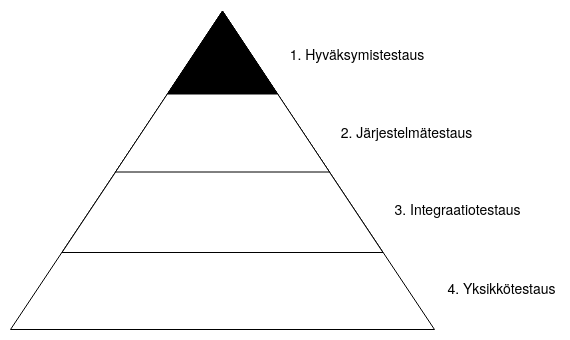
\includegraphics[width=0.8\textwidth]{assets/testauksen-tasot.png}
    \caption{Testauksen tasot pyramidin muodossa}
    \label{fig:testing-levels-pyramid}
  \end{figure}

  Pyramidimuodossa esitetyistä testauksen tasoista kaikkiin on mahdollista soveltaa testiautomaatiota.
  Testauksen menetelmien osalta hieman yksinkertaistaen valkolaatikkotestauksen alaisuuteen kuuluvat yksikkötestaus ja integraatiotestaus sekä mustalaatikkotestauksen alaisuuteen kuuluvat järjestelmätestaus ja hyväksyntätestaus.
  Pyramidimuodossa alimpana kuvataan aina yksikkötestaus, joka on tasoista atomisin ja myös luo vahvan pohjan kokonaisvaltaiselle testaamiselle.
  Noustessa pyramidissa ylöspäin, atomisuus häviää ja testattavana olevan kohteen laajuus sekä kompleksisuus kasvaa.
  Ylimpänä pyramidissa on hyväksymistestaus, joka on tarkoituksellista toteuttaa vaatimusmäärittelyn täyttävää valmista järjestelmää vastaan siten, että sen varmistetaan vastaavan loppukäyttäjän tarpeita.
  Monissa tapauksissa järjestelmätestauksen ja hyväksymistestauksen rajat saattavat olla epäselvät ja häilyvät.
  Tässä työssä hyväksymistestauksella tarkoitetaan käyttäjien hyväksyttämistestausta (UAT), jotta järjestelmätestauksen ja hyväksymistestauksen väliset eroavaisuudet tulevat lukijalle selkeästi esille.

  Hyväksymistestaus on tämän diplomityön keskiössä ja siihen liittyvää teoriaa esitetään vielä laajemmin hyväksymistestaus-luvussa \ref{ch:08_hyvaksymistestaus}.
  Seuraavissa kappaleissa esitetään vielä yksityiskohtaisemmin jokainen pyramidissa \ref{fig:testing-levels-pyramid} esitetty testauksen taso, jotta lukijalle muodostuisi käsitys erityisesti hyväksymistestauksen suhteesta muihin testauksen tasoihin.

  \subsection{Yksikkötestaus} \label{ch:07_yksikkotestaus}

    Yksikkötestauksen ajatuksena on testata ohjelmistotuotteen lähdekoodista löytyviä yksiköitä, kuten luokkia, funktioita tai moduleita.
    Yksikkötestaus toteutetaan ohjelmiston toteuttavia pienimpiä yksikköjä vastaan ja sen avulla pyritään validoimaan, että jokainen yksikkö toimii siten kuin ne on ohjelmistokehityksen aloitusvaiheessa suunniteltu toimimaan.
    Yksikkötestaus eroaa muista testauksen tasoista siinä, että sen voi suorittaa ainoastaan ohjelmistokehittäjät tai muut ohjelmiston lähdekoodiin perehtyneet henkilöt.
    Yksikkötestaus on näin ollen teknisesti valkolaatikkotestausta.
    Yksikkötestausta tarvitaan jotta voidaan pyrkiä varmistamaan, että ohjelmiston pienimmät yksiköt toimivat tarkoituksenmukaisella tavalla.

    Yksikkötestauksen toteuttamiseen käytetään pääsääntöisesti jotakin tarkoitusta varten räätälöityä testikirjastoa, joissa on keskenään yleensä hyvin samankaltainen rakenne.
    Yksikkötestaukseen tarkoitetuissa testikirjastoissa löytyy usein yksittäisen testitapauksen kuvaava tietorakenne, esimerkiksi luokka, sekä siihen usein kuuluvat alustus- ja lopetusfunktiot (setUp ja tearDown).
    Näiden lisäksi varsinainen testauskoodi toteutetaan pääsääntöisesti käyttäen niin sanottuja testikirjaston tarjoamia assert-funktioita, joiden avulla voidaan esimerkiksi varmistaa, onko jokin muuttuja tietyssä arvossa.

    Yksikkötestausta hyödynnetään usein myös ketterien menetelmien aihepiirissä, jossa ohjelmistotuotantoa voidaan toteuttaa muun muassa niin sanotulla testausvetoisella kehityksellä \ref{ch:07_testausvetoinen_kehitys}.
    Testausvetoisessa kehityksessä yksikkötestauksen osalta, ohjelmistokehittäjät laativat ensisijaisesti yksiköiden yksikkötestit ennen niiden toteuttamisen aloittamista.
    Ohjelmistotestauksen tasojen pyramidissa ja hyvin toteutetussa ohjelmistotestauksen monitasoisessa testauksessa tämä testauksen taso on usein kaikista laajin.
    Monitasoisessa testauksessa yksikkötestaus luo tärkeän pohjan testaamiselle kokonaisuutena ja antaa tietoa ohjelmiston pienimpien yksiköiden toimivuudesta.
    Yksikkötestaus on myös paljon käytetty ja tärkeä osa testiautomaatiossa, sillä se varmistaa sovelluksen yksiköiden suunniteltua toimintaa.

  \subsection{Integraatiotestaus} \label{ch:07_integraatiotestaus}

    Integraatiotestauksen ajatuksena on testata ohjelmistotuotteen toteuttavien eri komponenttien yhteentoimivuutta niiden rajapintojen osalta.
    Integraatiotestaus toteutetaan ohjelmiston suunnitelmaa ja mallia vastaan.
    Integraatiotestauksen onnistuminen luo validoitavan perustan ohjelmiston toimimiseen ja sen koostamiseen kokonaisena, eri komponenteista koostuvana järjestelmänä.
    Integraatiotestausta tarvitaan, jotta voidaan varmistaa sovelluksen yksiköiden yhteentoimivuus, joka ei pelkällä yksikkötestauksella tulisi muuten katetuksi.

    Integraatiotestauksen kohteita voivat olla esimerkiksi luokkien ja modulien väliset rajapinnat sekä web-sovelluksien api-ohjelmointirajapinnat.
    Integraatiotestauksen toteutuksen kannalta voidaan usein käyttää myös yksikkötestaukseen tarkoitettuja testikirjastoja ja työkaluja, mutta itse testitapauksien rakenne on silloin merkittävällä tavalla erilainen.
    Integraatiotestauksessa testitapauksien rakenteeseen tulee assert-funktioiden lisäksi myös tarvetta jäljitellä (englanniksi: mocking) rajapintojen tarjoamaa dataa.
    Rajapintojen datan jäljittelemiseen on olemassa useita valmiita työkaluja ja kirjastoja, joita integraatiotestauksen tapauksessa voi käyttää testitapauksien rakentamisen apuna.

    Integraatiotestauksen yhteydessä puhutaan usein myös niin sanotusta savutestauksesta, jonka tarkoituksena integraatiotestauksen yhteydessä on koostaa toistuva, esimerkiksi päivittäinen, koontiversio ohjelmistosta ja testata sen kriittisten komponenttien yhteentoimivuus.
    Integraatiotestaus on myös tärkeä osa testiautomaatiota, sillä sen avulla voidaan varmistaa sovelluksen yksiköiden, kuten esimerkiksi luokkien, komponettien tai modulien yhteentoimivuus.

  \subsection{Järjestelmätestaus} \label{ch:07_jarjestelmatestaus}

    Järjestelmätestauksen ajatuksena on testata kokonaista ja toimivaa järjestelmää, yhtenä suurena yksikkönä.
    Järjestelmätestaus toteutetaan usein eräänlaisena tulikokeena, erityisesti ohjelmiston vaatimuksia vastaan.
    Järjestelmätestausta tarvitaan, jotta voidaan varmistaa kokonaisen ohjelmiston toimivuus, jota ei muuten pelkällä yksikkötestauksella ja integraatiotestauksella saataisi täydellisellä varmuudella selville.
    Järjestelmätestaukseen liittyy laajasti erilaisia testattavia laadullisia ominaisuuksia, kuten toiminnallisuus, luotettavuus, käytettävyys, tehokkuus, ylläpidettävyys ja siirrettävyys \parencite{iso_9126-1_2001}.

    % Järjestelmätestauksen tyyppejä on yli 50, mutta tosiasiassa ohjelmistotestauksessa käytetään vain osaa niistä.
    % Tässä on osittainen lista ohjelmistotuotannossa yleisesti käytetyistä järjestelmätestauksen tyypeistä:

    % \begin{itemize}
    %   \item Regressiotestaus eli toistuva testaus
    %   \item Stressitestaus
    %   \item Toiminnallinen testaus
    %   \item Palautumistestaus
    %   \item Muutostestaus
    %   \item Käytettävyystestaus
    %   \item Alustatestaus
    % \end{itemize}

    <TODO: kirjoita tämä kappale paremmin...>

    Aiemmin testiautomaation tarkoitus kappaleessa \ref{ch:07_testiautomaation_tarkoitus} esitettiin, edellä mainituista laadullisista ominaisuuksista kaikki eivät sovellu hyvin testiautomaation avulla testattaviksi.
    Esitetyistä syistä johtuen, automatisoidulla järjestelmätestauksella voidaan testata edellä mainituista ominaisuuksista lähinnä ohjelmiston toiminnallisuutta, luotettavuutta ja tehokkuutta.
    Sen myötä testauksen tasona se voi olla testiautomaation teknisen toteutuksen kannalta jopa hyvin samanlainen kuin sitä spesifimpi hyväksymistestaus.
    Usein kuitenkin hyväksymistestauksessa paneudutaan erityisesti vaatimusmäärittelyyn ja asiakaslähtöiseen testaamiseen, kun taas järjestelmätestauksessa voidaan testata esimerkiksi myös järjestelmän tehokkuutta tai tietoturvaa.
    Tämä on tosin täysin riippuvainen vaatimusmäärittelystä, ja jos tehokkuus ja tietoturva ovat ohjelmiston asiakasvaatimuksia niin niiltä osin järjestelmätestaus ja hyväksymistestaus lomittuvat.
    Joissakin yhteyksissä järjestelmätestaus ja hyväksymistestaus esitetään jopa yhteisenä testauksen tasona, etenkin silloin kun testiautomaation kannalta ne muistuttavat kovasti toisiaan esimerkiksi edellä mainitulla tavalla.

    Järjestelmätestaus, osittain hyväksymistestauksen kanssa on erittäin merkittävä osa testiautomaatiosta, sillä sen avulla voidaan varmistaa kokonaisen järjestelmän vaadittu toiminnallisuus.

  \subsection{Hyväksymistestaus} \label{ch:07_hyvaksymistestaus}

    Hyväksymistestauksen ajatuksena on varmistaa toteutettavan ohjelmiston vaatimusten toimivuus erityisesti käytännön tilanteissa siten, että voidaan varmistaa vastaako ohjelmisto loppukäyttäjän tarpeita.
    Hyväksymistestaus toteutaan ohjelmiston toimintoja kuvaavaa vaatimusmäärittelyä ja loppukäyttäjistä sekä heidän tarpeista laadittuja käyttötapauksia vastaan.
    Samassa asiayhteydessä puhutaan usein myös niin sanotusta päästä päähän testauksesta (englanniksi: e2e, end-to-end).
    Päästä päähän testauksessa on tarkoituksena toteuttaa testaaminen siten, että polkuina ajateltuna, se sisältää kaiken siltä väliltä mitä loppukäyttäjä voi tarpeidensa saavuttamiseksi tehdä ja nähdä aloittaessaan ohjelmiston käytön ja lopettaessaan sen käytön.
    Testiautomaatio on erittäin hyödyllinen myös hyväksymistestauksen osalla, koska sillä voidaan automatisoida ohjelmiston validointi ja hyväksyminen, sekä estää puutteellisesti toimivan ohjelmiston julkaiseminen.
    Hyväksymistestausta tarvitaan myös, jotta voidaan testata ja validoida vaatimusten mukaisten ominaisuuksien toimivuus.

    <TODO: kirjoita tämä kappale paremmin...>

    Edellisessä kappaleessa käytiin jo hieman läpi järjestelmätestauksen ja hyväksymistestauksen samankaltaisuutta.
    Tässä on asiaa toisinpäin tarkasteltuna, osittainen lista ohjelmistotuotannossa havaittavista järjestelmätestauksen ja hyväksymistestauksen eroista, järjestelmätestauksen näkökulmasta:

    \begin{itemize}
      \item Painoarvo vaatimusmäärittelyssä
      \item Ohjelmistokehittäjien ja testaajien lisäksi myös sidosryhmät ja asiakkaat
      \item Testaus on vain lähinnä toiminnallista
      \item Testauksen syötteet tulevat suoraan käyttäjältä
      \item Testaus keskittyy arvioimaan täyttääkö ohjelmisto käyttäjän tarpeet
      \item A/B testaamisen mahdollisuus
      \item Hyväksymistestaus tapahtuu järjestelmätestauksen jälkeen
      \item Virheet käsitellään epäonnistumisina
    \end{itemize}

    Hyväksymistestaus, osittain järjestelmätestauksen kanssa on äärimmäisen hyödyllinen osa testiautomaatiosta, sillä sen avulla voidaan varmistaa kokonaisen järjestelmän toiminnallisuus ja verifioida, että se vastaa vaatimusmäärittelyä.
    Hyväksymistestauksen rooli testiautomaatiossa ja erityisesti jatkuvan integraation yhteydessä on indikoida voidaanko järjestelmä sellaisenaan julkaista loppukäyttäjille.

\section{Testitapaus ja testikokoelmat} \label{ch:07_testitapaus_ja_testikokoelmat}

  \begin{itemize}
    \item <TODO: Lisää testitapauksen esittely tähän>
    \item <TODO: Lisää testikokoelman esittely tähän>
    \item <TODO: Korosta testikokoelman ja käyttöliittymän näkymän yhteyttä tässä>
  \end{itemize}

\section{Jatkuva integrointi} \label{ch:07_jatkuva_integrointi}

  Testiautomaation rakentaminen manuaalisen testaamisen sijaan mahdollistaa sen liittämisen osaksi jatkuvaa integrointia.
  Lisäksi useissa yritysmaailman ohjelmistotuotannon prosesseissa pelkkä manuaalinen testaus kävisi selkeästi automatisoitujen koonti- tai julkaisuputkien periaatteita vastaan.
  Testiautomaation tarkoitus kappaleessa \ref{ch:07_testiautomaation_tarkoitus} aiemmin esitettiin testiautomaation ja manuaalisen testauksen eroa hyötyjen ja haittojen näkökulmasta.
  Testiautomaation toteuttaminen testitapauksien muodossa on jo itsessään testiautomaatiota, mutta käsitettä voidaan kuitenkin laajentaa, että myös jatkuva integrointi liittyy oleellisesti testiautomaation toteuttamiseen varsinkin nykyaikana ja ketteriin menetelmiin painottuvassa ohjelmistokehityksessä.

  Jatkuvalla integroinnilla tarkoitetaan versiohallintaisessa ohjelmistokehityksessä väistämättömän integrointiprosessin muuntamista jatkuvaksi.
  Ohjelmistokehityksessä integrointiprosessi tulee vastaan, kun eri ohjelmistokehittäjät tai tiimit toteuttavat muutoksia tai uusia ominaisuuksia kehitettävänä olevaan ohjelmistotuotteeseen.
  Tällaisessa tilanteessa yksittäiset ohjelmistokehittäjät tai tiimit toteuttavat uutta ohjelmakoodia toisistaan irrallaan siihen asti kunnes muutokset tai ominaisuudet tulee yhdistää yhdeksi kokonaiseksi kehityksen kohteena olevaksi ohjelmistotuotteeksi, jota prosessina kutsutaan integrointiprosessiksi.
  Jatkuvan integroinnin tarkoituksena on nopeuttaa integrointiprosessia ja muuttaa ohjelmistokehityksessä käytössä olevia periaatteita siten, että siitä tulee luonnostaan jatkuvaa.
  Jatkuvan integroinnin toteuttaminen tarvitsee teknisesti sen mahdollistavan versionhallintajärjestelmän ja varsinaisen jatkuvan integroinnin palvelimen.

  \begin{figure}[H]
    \centering
    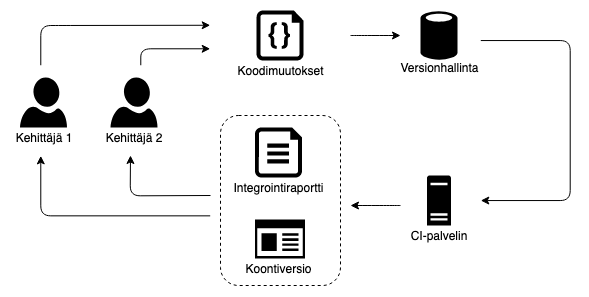
\includegraphics[width=0.8\textwidth]{assets/jatkuva-integrointi.png}
    \caption{Jatkuvan integroinnin perusperiaate on iteratiivinen}
    \label{fig:jatkuva-integrointi}
  \end{figure}

  Esimerkkinä versionhallintajärjestelmänä voidaan käyttää nykyaikana suosittua git versionhallintaohjelmistoa ja jatkuvan integroinnin palvelimena esimerkiksi GoCD ohjelmistoa.
  Perusideana jatkuvassa integraatiossa on konfiguroida jatkuvan integraation mahdollistava ohjelmisto siten, että se kuuntelee versionhallintaan tulevia muutoksia ja suorittaa integrointiprosessin jatkuvasti sellaisia huomattuaan.
  Versionhallintaan tulevat muutokset voidaan jatkuvan integraation osalta kuunnella ajastetusti tietyin väliajoin tai oikeasti jatkuvasti käyttämällä esimerkiksi web-koukkuja, jotka tiedottavat jatkuvan integraation palvelimelle versionhallintaan saapuneista muutoksista.
  Jatkuvan integroinnin yhden iteraatiokerran integrointiprosessin tuloksena on tarkoituksena tarjota periaatteeltaan sama lopputulema kuin mitä se olisi manuaalisella integrointiprosessillakin.
  Jatkuva integroinnin mahdollistava konfiguraatio sisältää jonkinlaisen koontiputken tai koontiputkia, joissa rakennetaan koontiversio kehitettävän ohjelmiston lähdekoodeista.
  Koontiputki voi sisältää esimerkiksi ohjelman lähdekoodien kääntämisen asiaan sopivalla kääntäjällä.
  Kääntämisen lisäksi koontiputkeen on tässä vaiheessa erittäin kannattavaa yhdistää testiautomaatiota, kuten esimerkiksi automaattiset yksikkötestit ennen kääntämistä ja hyväksymistestit kääntämisen jälkeen.

  Jatkuvan integroinnin yhteydessä suoritettavat testikokoelmat ja niiden sisältävät testitapaukset ovat erittäin järkevää toteuttaa, sillä ne esimerkiksi parantavat ohjelmistokehityksen ja lopputuotteen luotettavuutta ja laatua.
  Jatkuvan integroinnin sisältämästä koontiputkesta saadaan hyödyllistä palautetta ja raportteja integrointiprosessin onnistumisesta, joka voidaan ohjata pääasiassa ohjelmistokehittäjille sekä myös muillekin sidosryhmille.
  Jatkuvalla integroinnilla itsessään on myöskin paljon sen käyttöönoton antamia hyötyjä, kuten esimerkiksi toteutettujen muutosten tai toimintojen integrointitiheyden kasvattamisen tuomat edut.
  Jos muutosten tai toimintojen integroiminen on perinteisessä ohjelmistokehitetyksessä tehty esimerkiksi viikoittain, niin jatkuva integroiminen korjaa sen tuomat haasteet turhan laajasta integrointiprosessista ja mahdollisesta ohjelmistokoodin hajoamisesta.
  Tällaisissa tapauksissa ohjelmistokoodi voi sisältää epäyhteensopivia moduleita tai muita rajapintoja sekä mahdollisuuden käännettävien lähdekoodien kääntämisen onnistumisesta.

\section{Testausvetoinen kehitys} \label{ch:07_testausvetoinen_kehitys}

  Perinteisesti testiautomaatio on soveltunut hyvin vain vakaille ohjelmistoille ja niiden regressiotestaamiseen.
  Nykypäivänä ohjelmistokehitys on siirtynyt suunnitelmapohjaisista prosesseista iteroiviin ketteriin ohjelmistotuotannon prosesseihin.
  Näihin testiautomaatio on soveltunut huonosti, kun testattavaa ohjelmistoa tai lisättyä toiminnallisuutta ei ole vielä olemassa.
  Tähän ongelmaan on kehittynyt niin sanottu testausvetoinen kehitys, jossa testitapaukset suunnitellaan ja toteutetaan ennen varsinaisen ohjelmiston tai toiminnon toteutuksen toteuttamista.

  \begin{figure}[H]
    \centering
    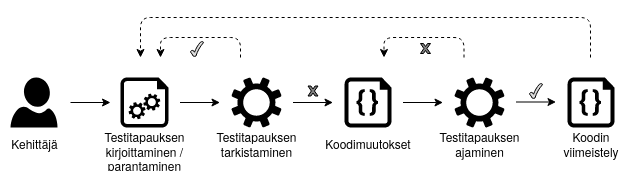
\includegraphics[width=0.8\textwidth]{assets/testausvetoinen-kehitys.png}
    \caption{Testausvetoisen kehityksen vaiheet}
    \label{fig:testausvetoinen-kehitys}
  \end{figure}

  Testausvetoinen kehityksen sisältämät vaiheet \ref{fig:testausvetoinen-kehitys} alkavat testitapauksien luomisesta ja niiden tarkastamisesta.
  Tarkastaminen tapahtuu siten, että testitapaukset ajetaan oletuksella, että niiden täytyy tässä vaiheessa epäonnistua.
  Alkuvaiheen testitapauksien luomisen jälkeen ohjelmistkehittäjät kehittävät ohjelmistoa tekemällä siihen muutoksia ihanteellisesti testitapauksien kokoisia paloja kerrallaan.
  Kun koodimuutoksia on syntynyt, riippuen ohjelmistotuotannossa käytössä olevasta integrointiprosessista, ajetaan testitapaukset manuaalisesti tai jatkuvan integroinnin avulla.
  Integrointiprosessista saadaan palautetta, jonka mukaan ohjelmakoodia korjataan tai viimeistellään.
  Testausvetoisella kehityksellä pyritään nopeuttamaan ohjelmistokehitysprosessia verrattuna perinteisiin ohjelmisttuotannon menetelmiin.
  Tämän jälkeen testausvetoista kehitystä käyttävässä ohjelmistotuotantoprosessissa siirrytään takaisin testitapauksien luomiseen ja parantamiseen sekä aloitetaan toinen iteraatiokierros mikäli ohjelmisto ei vielä ole valmis.

  Testausvetoisessa kehityksessä testitapaukset siis laaditaan jo varhaisessa vaiheessa jolloin niiden tekeminen saattaa usein olla liiketoiminnan näkökulmasta helpommin perusteltavaa liiketoiminnan johdolle.
  Tämän lisäksi testitapauksien kirjoittaminen etukäteen luo kattavat testikokoelmat jo alusta alkaen, joita voidaan hyödyntää iteratiivisesti ohjelmistotuotteesta riippuen usein hyvinkin pitkään, etenkin jos niihin tehdään tarvittavaa hienosäätöä ohjelmistokehityksen aikana.
  Ohjelmistokehittäjät voivat kehittää helposti hallittavissa olevia testitapauksien rajaavia kokonaisuuksia, jolloin ohjelmistotuote valmistuu ikään kuin pala kerrallaan.
  Itse ohjelmistkehitys on siis iteratiivista ja näin ollen testitapauksien suorittamisesta saadaan palautetta ja raportointia koko ohjelmistotuotantoprosessin aikana.
  Testausvetoinen kehitys kuuluu ohjelmistotuotannossa vahvasti ketterien menetelmien alaisuuteen ja on kasvattanut suosiotaan ketterien menetelmien mukana.

\chapter{Hyväksymistestaus} \label{ch:08_hyvaksymistestaus}
  Tässä luvussa esitetään perusteet ja tarvittavat tiedot hyväksymistestauksesta, johon testauksen tasoista tässä diplomityössä keskitytään.
Ensin esitetään hyväksymistestauksen tarkoitus, jonka jälkeen keskitytään hyväksymistestausvetoiseen kehitykseen ja sen esittelemiseen ohjelmistotuotannollisena menetelmänä.
Hyväksymistestausvetoisen kehityksen jälkeen käydään läpi tässä diplomityössä käytettyä ja lähes de facto testialustaa, Robot frameworkia, hyväksymistestauksen testitapauksien rakentamiseen.
Robot frameworkin perusteiden jälkeen esitetään hyväksymistestauksen testitapauksien laatiminen käyttäen Robot frameworkia sekä esitetään web-sovelluksien erityispiirteitä jotka on huomioitava hyväksymistestauksessa.
Hyväksymistestaksen perusteiden ymmärtämistä tarvitaan työn toteutusvaiheessa, jossa esitetään korkealla tasolla asiakasyritykselle toteutettua hyväksymistestausta ja sen automaatiota.
Lopuksi esitetään yleisestikin ottaen testitapauksiin tärkeästi liittyvä priorisointiongelma ja käydään läpi sen eri ratkaisumalleja, keskittyen erityisesti tässä diplomityössä myöhemmin esitettävään priorisointiin painotetun verkon avulla.

\section{Hyväksymistestauksen tarkoitus} \label{ch:08_hyvaksymistestauksen_tarkoitus}

  Hyväksymistestauksen tarkoituksena on varmistaa toteutettavan ohjelmiston vaatimusten toimivuus erityisesti käytännön tilanteissa siten, että voidaan varmistaa vastaako ohjelmisto loppukäyttäjän tarpeita.
  Hyväksymistestaus antaa vastauksen siihen, toimiiko toteutettu järjestelmä loppukäyttäjän tarpeiden mukaisesti ja loppukäyttäjän näkökulmasta oikein.
  Hyväksymistestauksen sanotaan olevan muodollista testaamista, jossa käyttäjän tarpeet, vaatimukset ja liiketoimintaprosessit otetaan huomioon selvittäessä täyttääkö järjestelmä hyväksymisen kriteerit ja sallii käyttäjän, asikkaiden tai muun autorisoidun tahon päättää hyväksytäänkö järjestelmä \parencite{istqb_glossary_nodate}.
  Ohjelmistotestauksen tekniikoiden näkökulmasta hyväksymistestaus on mustalaatikkotestausta, eli sitä testataan tietämättä sen teknisestä toteutuksesta.
  Hyväksymistestauksen painoarvo on asiakaperusteisessa vaatimusmäärittelyssä ja loppukäyttäjän tarpeiden kartoittamisessa.
  Testiautomaation osalta hyväksymistestausta varten voidaan rakentaa testitapaukset, joiden avulla voidaan keskittyä varmistamaan loppukäyttäjille tarpeellisten toimintojen toteutuminen testitapauksien suorittamisen jälkeen.
  Hyväksymistestauksen osalta testitapauksia voidaan toteuttaa niin sanotulla päästä päähän -periaatteella, jossa testattavaa järjestlemää testataan siten kuin loppukäyttäjä sitä käyttää.
  Hyväksymistestauksessa ei anneta suurta painoarvoa kosmeettisille tai kirjoitusvirheille, vaan pyritään selvittämään loppukäyttäjille oleellisten ja tarpeellisten toimintojen toteutuminen.

  Hyväksymistestaus on aiemmin esitetyistä testauksen tasoista \ref{ch:07_testauksen_tasot} viimeinen ja sen suorittamisen jälkeen saadaan tieto siitä onko järjestlemä toteutuksen osalta sellaisenaan valmis julkaistavaksi.
  Perinteisesti hyväksymistestauksen lähtökohtia ovat selvät hyväksymisvaatimukset sekä julkaisukelpoinen toteutus joka voi sisältää vain kosmeettisia virheitä.
  Hyväksymisvaatimukset voivat olla esimerkiksi liiketoiminnallisia käyttötapauksia, prosessivirtauskaavioita sekä ohjelmiston vaatimusmäärittely.
  Testiautomaatiota varten käytettävästä testialustasta riippuen hyväksymistestauksen käyttötapaukset voidaan muodostaa joko osittain tai suoraan testitapauksiksi.
  Hyväksymistestaukseen usein osallistuu ohjelmistokehittäjien lisäksi myös muut sidosryhmät ja loppukäyttäjät.
  Keskeistä on, että loppukäyttäjiltä hankitaan tieto tarvittavista ja toteutettavista ominaisuuksista, kun taas muut sidosryhmät kuten esimerkiksi johtoryhmä voivat tehdä liiketoiminnallisia päätöksiä hyväksymistestauksen onnistumisen osalta ja esimerkiksi peruuttaa julkaisun.
  Hyväksymistestaus antaa mahdollisuuden korjata usein liiketoiminnalisestakin näkökulmasta merkittävät toiminalliset virheet ennen järjestelmän julkaisua loppukäyttäjille.

  Kehittäjien käsitys järjestelmän toiminnallisuudesta ja sen vaatimuksista voi olla usein hyvinkin erilainen kuin loppukäyttäjien.
  Hyväksymistestauksen avulla voidaan tätä lievittää tätä ongelmaa, ja saattaa ohjelmistokehittäjät loppukäyttäjien kanssa vaatimusmäärittelyn suhteen samalle sivulle.
  Testiautomaation avulla toteutettavalla toistuvalla hyväksymistestauksella varmistetaan, että järjestelmä toteuttaa loppukäyttäjän tarpeet vielä järjestlemään tehtyjen muutoksien jälkeenkin.
  Hyväksysmistestauksen testitapaukset tarkoituksenmukaisesti heijastavat suoraan loppykäyttäjien tarpeita, joka on iso etu sillä sen avulla ohjelmistokehittäjät ja muut sidosryhmät voivat tehokkaasti varmistaa järjestlemän valmiuden ja tilan.
  Hyväksymistestauksella siis saadaan katsaus ohjelmiston valmiudesta sen vaatimuksiin ja loppukäyttäjien toiminnallisiin tarpeisiin nähden.

\section{Hyväksymistestausvetoinen kehitys} \label{ch:08_hyvaksymistestausvetoinen_kehitys}

  Hyväksymistestausvetoisen kehityksen (englanniksi: ATDD, acceptance test driven development) tarkoituksena, kuten testausvetoisessakin kehityksessä \ref{ch:07_testausvetoinen_kehitys} on toteuttaa ohjelmistotuotannollinen prosessi laatien toistettavasti suoritettavat testitapaukset ennen ohjelmiston varsinaista toteutusta.
  Hyväksymistestausvetoisessa kehityksessä tämä tarkoittaa käytännössä sitä, että ennen toteutusta luodaan tarvittavat ohjelmiston asiakasvaatimuksia palvelevat hyväksymistestit, jotka ohjelmiston on tarkoitus läpäistä sen julkaisemisen hyväksymiseksi.
  Hyväksymistestausvetoisen kehityksen sanotaan olevan yhteistyöhön perustuva lähestymistapa kehitykseen, jossa tiimi ja asiakkaat käyttävät asiakkaiden oman ympäristön kieltä ymmärtääkseen heidän vaatimukset, jotka muodostavat pohjan komponentin tai järjestelmän testaamiseen \parencite{istqb_glossary_nodate}.
  Tarvittavat ohjelmiston hyväksymistestit suoritetaan iteratiivisesti ohjelmistokehitysprosessin aikana ja se tarkoittaa käytännössä jatkuvan integraation \ref{ch:07_jatkuva_integrointi} ottamista käyttöön ohjelmistokehityksessä.
  Hyväksysmistestausvetoinen kehitys on erittäin hyödyllinen ohjelmistokehityksessä käytetty menetelmä, sillä kehitysvaiheessa on aina tarkasti tiedossa vastaako ohjelmiston tila asiakasvaatimuksia ja kuinka hyvin se niiden täyttämisessä onnistuu.

  \begin{figure}[H]
    \centering
    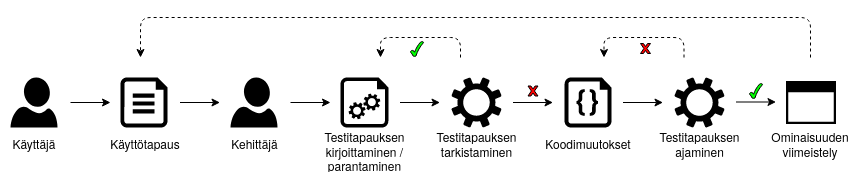
\includegraphics[width=0.8\textwidth]{assets/hyvaksymistestausvetoinen-kehitys.png}
    \caption{Hyväksymistestausvetoisen kehityksen vaiheet}
    \label{fig:hyvaksymistestausvetoinen-kehitys}
  \end{figure}

  Hyväksymistestausvetoinen kehitys voidaan luokitella ketteräksi ohjelmistokehitysmenetelmäksi, kuten sen yläkäsitteenä oleva testausvetoinen kehityskin \ref{ch:07_testausvetoinen_kehitys}.
  Hyväksymistestausvetoinen kehitys on testausvetoisen kehityksen kanssa perusperiaatteeltaan samanlainen, mutta ennen ohjelmistokehityksen aloitusta asiakasvaatimukset kartoitetaan ja ohjelmiston hyväksyttävyys määritetään.
  Hyväksymistestitapaukset kirjoitetaan testausvetoisen kehityksen mukaisesti ensin ja ohjelmistokehitys itsessään noudattaa iteratiivisesti testausvetoista kehitystä, vaikkakin hyväksymistestaus itsessään on perinteisesti vaatinut lähes valmista järjestlemää.
  Asiakasvaatimukset määritetään usein käyttötapauksien muotoon, ja riippuen testialustasta ne voidaan kirjottaa testitapauksien muotoon niitä vahvasti hyödyntäen.
  Hyväksymistestausvetoisessa kehityksessä ohjelmistokehitystä siis ohjaavat asiakasvaatimukset ja loppukäyttäjien tarpeiden toteutuminen, jotka ovat hyvin usein toiminallisia vaatimuksia.
  Hyväksymistestausvetoisessa kehityksessä mitataan jatkuvasti iteroiden käyttötapauksien muodossa validoitavien haluttujen ominaisuuksien toteutumista.
  Perusperiaate on kirjoittaa asiakasvaatimus tai käyttötapaus testitapauksen muotoon, toteuttaa testitapaus, ajaa testitapaus läpäisemättömänä, toteuttaa ominaisuus, ajaa testitapaus läpäisevänä, refaktoroida toteutus ja siirtyä takaisin seuraavaan käyttötapaukseen.
  Käyttötapaus koostuu rakenteellisesti usein tilanteesta, motivaatiosta ja halutusta lopputuloksesta.
  Esimerkki käyttötapauksesta voi olla: \emph{käyttäjänä, haluan sisäänkirjautumisen jälkeen voida avata premium ominaisuudet tekemällä sovelluksensisäisen oston}.

  Hyväksymistestausvetoisessa kehityksessä hyväksymistestit on hyödyllistä pilkkoa pieniin hallittaviin kokonaisuuksiin, jolloin voidaan iteratiivisesti toteuttaa valmiiksi tietyn testitapauksen mukainen ominaisuus, joka vastaa jotakin käyttötapausta tai loppukäyttäjän tarvetta.
  Hyväksymistestauksessa testitapaus voi olla esimerkiksi käyttäjän tietojen muuttuminen varmistaminen, kuten tason läpäiseminen pelisovelluksessa, joka muuttaa käyttäjän edistystä.
  Hyväksymistestausvetoisen kehityksen tarkoituksena menetelmänä on onnistua vastaamaan loppykäyttäjän tarpeisiin tehokkaasti ja hyvin ottamalla tarpeet huomioon jo ennen toteutuksen aloittamista.
  Menetelmän avulla myös luodaan ymmärrystä ohjelmistotuotteen valmiuden määritelmästä kun eri sidosryhmän voidaan saada sen suhteen samalle aaltopituudelle.
  Hyväksymistestausvetoinen kehitys on lisäksi erittäin hyödyllistä, sillä jatkuva testaaminen antaa mahdollisuuden haluttujen ominaisuuksien toteutumisen validoimiselle menetelmän jokaisen iteraation koontiversiossa.

\section{Web-sovelluksien erityispiirteet} \label{ch:08_websovelluksien_erityispiirteet}

  Web-sovelluksilla on omia erityispiirteitä, jotka vaikuttavat testitapauksien laatimiseen.
  Nykypäivänä web-sovellukset ovat kasvaneet kompleksisuudessa ja front-end puolen toteutuksesta tarkasteltuna web-sovellukset usein muistuttavat jo perinteisiä työpöytäsovelluksia.
  Web-sovelluksia päivitetään nykyään tiheään tahtiin ja niille on suuri tarve luoda testiautomaatiota, jota hyödyntäen voidaan varmistaa että ne toimivat oikein muutoksien jälkeenkin.

  Hyväksymistestauksen priorisoimisen osalta tärkeä web-sovelluksien erityispiirre liittyy käyttöliittymiin ja dokumenttiobjektimalliin, DOM.
  Dokumenttiobjektimallin avulla verkkoselaimet renderöivät käyttöliittymän ja siinä näkyvän sisällön.
  Tämän lisäksi dokumenttiobjektimalli mahdollistaa käyttöliittymässä olevien elementtien valitsemisen, jota hyödynnetään myös testitapauksien kirjoittamisessa.

  Navigointi ja navigointiketjut ovat myös yksi web-sovelluksien erityispiirre.
  Historiallisesti verkkosivuilla navigointi tapahtui niin kutsuttujen hyperlinkkien avulla, verkkosivujen itse ollessa hypertekstiä.
  Tämä historiallinen lähestymistapa on edelleen käytössä ja web-sovelluksissa on lähes poikkeuksetta useita hyperlinkkejä joiden avulla navigoiminen luo erityisiä navigointiketjuja, joissa edelliseen sivuun tiedetään palata.
  Hyperlinkkien avulla tapahtuva navigointi ja navigointiketjut on erityispiirre, joka on hyvä tiedostaa myös hyväksymistestauksen testitapauksia rakentaessa.

  Web-sovelluksien syötteet ja niiden yhteyteen liittyvä tietoturva ovat myös yksi niiden erityispiirre joka vaatii suurta huomiota.
  Web-sovelluksien syötteisiin on perinteisesti liittynyt paljon haavoittuvuuksia, kuten esimerkiksi XSS-hyökkäykset ja SQL-injektiot.
  Web-sovelluksien hyväksymistestauksen testitapauksiin on hyvä sisällyttää syötteisiin liittyvää testaamista, joissa tietoturva pidetään mielessä.

  Erilaisia web-sovelluksen loppukäyttäjien asiakasympäristöjä on huikean paljon, joka kannustaa moniselaimellisen testauksen rakentamiseen.
  Näissä ympäristöissä on omat verkkoselaimensa, näyttöresoluutio ja selainasetukset, jotka saavat saman sovelluksen toimimaan eri tavoilla eri ympäristöissä ja luovat siten usein jopa päänvaivaa ohjelmistokehittäjille.
  Etenkin web-käyttöliittymiin keskittyessä testitapauksiin on hyvä sisällyttää erilaisia näyttöresoluutioita, kuvankaappauksien ottamista ja selainasetuksista esimerkiksi Javascript-ominaisuuksien estäminen.

  Web-sovelluksien käyttöliittymien testaaminen ja yleisestikkin ottaen käyttöliittymien testaaminen on perinteisesti tapahtunut manuaalisesti.
  Nykyään web-sovelluksia voidaan testata niin sanotun päätteettömän testauksen keinoin.
  Web-sovelluksien päätteettömässä testauksessa verkkoselaimen, näyttöresoluution ja selainasetuksien muodostamaa asiakasympäristö rakennetaan virtualisoinnin avulla.
  Virtualisoinnista vastaa joko verkkoselain itse tai voidaan käyttää UNIX järjestelmissä x-näyttöpalvelimen protokollan toteuttavaa virtualisointiratkaisua, esimerkiksi Xvfb.
  Virtualisoitu asiakasympäristö rakennetaan siten, että se päätteettömänä vastaa täysin päätteellistä vaihtoehtoa, ja siitä voidaan ottaa esimerkiksi kuvankaappaus vaikka mitään ihmisen astittavaa ei ole näkyvillä.

\section{Hyväksymistestauksen työkaluja} \label{ch:08_hyvaksymistestauksen_tyokaluja}

  Tässä kappaleessa esitetään diplomityötä tehdessä käytettyjä ja osin myös varsin yleisiä testiautomaation mahdollistavia työkaluja, kukin omassa alikappaleessaan.
  Ensin esitetään hyväksymistestauksen automatisoimisen kannalta kaikista tärkeimmät työkalut, eli testikehyksenä käytettävä Robot framework ja web-sovelluksien interaktioiden automatisoimisen mahdollistava Selenium kirjasto.
  Lisäksi esitetään kolme muuta tärkeää työkalua joiden avulla voidaan rakentaa kokonainen ohjelmistotuotannon prosessiin intergroitavissa oleva hyväksymistestausjärjestelmä.
  Toteutuksessa GoCD vastaa jatkuvan integroinnin tarjoamisesta, Xvfb vastaa päätteettömän testauksen tarjoamisesta ja Docker vastaa työkalujen virtualisoimisesta ja säiliöinnistä, jolloin työkaluista saadaan luotua yhtenäinen kokonaisuus.

  \subsection{Robot Framework} \label{ch:08_robot_framework}

    Robot framework on geneerinen avoimen lähdekoodin testausalusta hyväksymistestaukseen, hyväksymistestausvetoiseen kehitykseen ja robotisten prosessien automaatioon \parencite{noauthor_robot_nodate}.
    Testialustana Robot frameworkilla on helposti ymmärrettävä, luettava ja selkeä avainsanaperustainen syntaksi.
    Testialustan etuna on helppo lähestyttävyys ja sen pohjalle rakennettujen testitapauksien ymmärtäminen ei vaadi ohjelmakoodin ymmärtämistä.
    Robot framework on Python-perustainen testialusta joka on helppo asentaa, sitä on helppoa ymmärtää, sillä on kattava dokumentaatio ja se on helppoa ottaa käyttöön.

    Robot frameworkissa on sisäänrakennettu tuki ulkoisille kirjastoille ja dokumentaatiosta löytyy paljon tietoa omien avainsanojen ja omien kirjastojen tekemiseen.
    Lisäksi Robot framework on todella suosittu ja sisäänrakennettujen ominaisuuksien lisäksi ulkoisia kolmansien osapuolien kirjastoja löytyy alustalle paljon.
    Robot framework tukee muuttujien käyttöä testitapauksien rakentamisessa, joilla voi lisätä hieman kompleksisuutta ja logiikkaa omiin testitapauksiin.
    Robot frameworkista löytyy myös tuki dataperustaisien testitapauksien rakentamiseen, joille annetaan eri syötteitä sisältävää testidataa.
    Testitapauksia voi myös ryhmitellä testikokoelmiin käyttämällä tägejä testitapauksien sisällä.

    \begin{figure}[H]
      \centering
      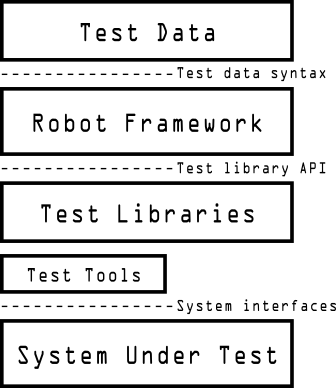
\includegraphics[width=0.4\textwidth]{assets/robot-arkkitehtuuri.png}
      \caption{Robot framework alustan arkkitehtuuri}
      \label{fig:robot-architecture}
    \end{figure}

    Robot frameworkillä rakennettuja testitapauksia voidaan ajaa komentoriviltä robot komennolla.
    Testitapauksien ajaminen tulostaa komentoriville yksinkertaisen raportin testitapauksen onnistumisesta ja lisäksi tallettaa varsin yksityiskohtaisen ja selkeän testitaportin ajetuille testitapauksille.
    Testiraportit ovat erittäin hyvin tehtyjä ja html-pohjaisia, joka tarkoittaa että ne voidaan helposti integroida osaksi jatkuvan integraation koontiputkia.

    Yhtenä heikkoutena Robot frameworkissa on tuen puuttuminen ohjelmistokieliperustaisissa testikehyksissä löytyville kontrollirakenteille, joita esiintyy esimerkiksi yksikkötestaukseen tarkoitetuissa testikehyksissä.
    Robot framework on selkeästi vain hyväksymistestauksen testitapauksien rakentamista varten tarkoitettu testialusta ja siinä se on erinomainen vaihtoehto testitapauksien rakentamiseen.

  \subsection{Selenium} \label{ch:08_selenium}

    % TODO: Kirjoita tämä kappale

    \begin{itemize}
      \item Mikä se on?
      \item Mihin sitä käytetään?
      \item Mitä hyötyjä siitä saadaan?
      \item Sisäinen rakenne / yksityiskohtainen esittely
      \item (Mitä heikkouksia siinä on?)
      \item Yhden lauseen yhteenveto
    \end{itemize}

  \subsection{Xvfb} \label{ch:08_xvfb}

    % TODO: Kirjoita tämä kappale

    \begin{itemize}
      \item Mikä se on?
      \item Mihin sitä käytetään?
      \item Mitä hyötyjä siitä saadaan?
      \item Sisäinen rakenne / yksityiskohtainen esittely
      \item (Mitä heikkouksia siinä on?)
      \item Yhden lauseen yhteenveto
    \end{itemize}

  \subsection{GoCD} \label{ch:08_gocd}

    % TODO: Kirjoita tämä kappale

    \begin{itemize}
      \item Mikä se on?
      \item Mihin sitä käytetään?
      \item Mitä hyötyjä siitä saadaan?
      \item Sisäinen rakenne / yksityiskohtainen esittely
      \item (Mitä heikkouksia siinä on?)
      \item Yhden lauseen yhteenveto
    \end{itemize}

  \subsection{Docker} \label{ch:08_docker}

    % TODO: Kirjoita tämä kappale

    \begin{itemize}
      \item Mikä se on?
      \item Mihin sitä käytetään?
      \item Mitä hyötyjä siitä saadaan?
      \item Sisäinen rakenne / yksityiskohtainen esittely
      \item (Mitä heikkouksia siinä on?)
      \item Yhden lauseen yhteenveto
    \end{itemize}

\section{Testitapauksien määrittäminen} \label{ch:08_testitapauksien_maarittaminen}

  Testitapaus on testiautomaation näkökulmasta, määritelty toimenpiteiden, ehtojen ja muuttujien joukko, joka suorittamalla voidaan verifioida ominaisuus tai toiminnallisuus ohjelmistosta.
  Testitapauksiin liittyy oleellisesti testikokoelman käsite, joka tarkoittaa samaan kontekstiin kuuluvista testitapauksista muodostettua joukkoa.
  Tässä diplomityössä keskitettyyn hyväksymistestaukseen liittyen testitapaukset kirjoitetaan usein käyttötapauksien muodossa.
  Lisäksi hyväksymistestauksen priorisoimiseen painotetun verkon avulla on suositeltavaa suunnitella ja rakentaa testitapaukset näkymä ja siirtymäperusteisesti, jotta matemaattisia verkkoja voidaan kunnolla hyödyntää.

  Testitapauksen perusformaatti koostuu lähtötilanteesta, laukaisijasta ja verifikaatiosta.
  Lähtötilanteessa oletetaan jotakin ja seuraavassa vaiheessa seurataan kun jokin ehto tapahtuu, jonka jälkeen voidaan tarkistaa seuraus ja verifioida onko se oletuksen mukainen.
  Testitapauksien yleisiä tavoitteita ovat: yksinkertaisuus, läpinäkyvyys, käyttäjätietoisuus, epätoistuvuus, olettamattomuus, kattavuus, tunnistettavuus, jälkensä puhdistava, toistettava, syvyyttömyys ja atomisuus.

  \noindent\begin{minipage}{\linewidth}
  \renewcommand{\lstlistingname}{Koodi}
  \lstinputlisting[
    caption={Esimerkki testitapauksesta Robot frameworkillä},
    label=code:robot-framework-testitapaus,
    numbers=left
  ]{assets/robot-framework-testitapaus.robot}
  \end{minipage}

  Robot Frameworkin perustaja on kirjoittanut laajan ohjeistuksen siitä, miten Robot Frameworkiä käyttäen luodaan hyviä testitapauksia \parencite{klarck_how-to-write-good-test-cases_2019}.
  Klärckin ohjeistuksen pohjalta on huomioitavaa erityisesti testikokoelmien, testitapauksien ja avainsanojen nimeäminen jonka kuuluisi olla selkeää, kuvaavaa ja ytimekästä.
  Dokumentaation määrää testitapauksissa tulisi rajoittaa, sillä hyvin kirjoitetut testitapaukset ovat Robot frameworkiä käyttäen selkeitä jo sellaisenaan.
  Dokumentaatiota kuuluisi lisätä lähinnä vain testikokoelmiin yleisellä tasolla.
  Testikokoelmat kuuluisi sisältää vain toisiinsa liittyviä testejä ja testitapauksien sekä avainsanojen tulisi olla sellaisinaan selkeästi ymmärrettäviä.
  Muuttujien käyttöä suositellaan kapsuloimaan pitkiä ja kompleksisia arvoja, mutta arvojen syöttäminen ja palauttaminen muuttujia hyödyntäen tulisi pitää pois testitapauksien tasolta.

\section{Priorisointiongelma} \label{ch:08_priorisointiongelma}

  Testitapauksien priorisointi on kustannussyistä tai resurssien optimoinnin kannalta erittäin tärkeää.
  Ohjelmistotestauksessa on hyvä tiedostaa, että ohjelmistotuotetta ei usein voida testata täydellisesti, joka nostaa esiin tarpeen tärkeimpien testitapauksien löytämisestä.
  Priorisoinnin toutettamisen tärkeys korostuu erityisesti silloin kun kohdejärjestelmä on kompleksinen ja toimminallisia ominaisuuksia on paljon.

  Priorisoinnista saatavia hyötyjä:
  \begin{itemize}
    \item Tärkeät ongelmat löydetään aikaisin
    \item Testitapauksien suorittamisen järjestäminen
    \item Epäoleelliset testitapaukset voidaan jättää toteuttamatta
    \item Kustannuksia ja resursseja säästyy
    \item Käytännönläheisyys
    \item Korkean prioriteetin testitapauksiin voidaan käyttää huolellista suunnittelua
  \end{itemize}

  % TODO: Lisää tekstiä tähän kappaleeseen. Eheyden kannalta tärkeä kappale!
  <TODO: kirjoita tähän lisää tekstiä...>

  Priorisointiongelmaan on olemassa useita erilaisia lähestymistapoja ja menetelmiä, kuten esimerkiksi heuristinen priorisointi tai MoSCoW menetelmä.
  Tässä diplomityössä priorisointiin käytetään kuitenkin matemaattista painotettuihin verkkoihin perustuvaa lähestysmistapaa, joka on uudenlainen tämän diplomityön tuotteena kehittynyt menetelmä priorisointiongelman ratkaisemiseen.

\chapter{Verkkoteoria} \label{ch:09_verkkoteoria}
  Tässä luvussa käsitellään työhön keskeisesti kuuluvan verkkoteorian perusteet käydää huolellisesti läpi erityisesti työssä käytettävät osat.
Työssä sovelletaan erityisesti verkkoteorian painotettua verkkoa sekä verkkoteoriassa esiintyvän lyhimmän polun ongelmaan kehitettyä Djikstran algoritmia.
Verkkoteoria itsessään on osa diskeettiä matematiikkaa.

\section{Matemaattisten verkkojen tarkoitus} \label{ch:09_matemaattisten_verkkojen_tarkoitus}

  Matemaattisten verkkojen tarkoituksena on mallintaan parittaisia riippuvuuksia verkkomaisessa objektijoukossa.
  Verkkoteoriassa peruskäsitteitä ovat itse \emph{verkko} eli \emph{graafi}, joka muodostuu \emph{solmuista} ja niiden välisiä riippuvuuksia esittävistä \emph{kaarista} tai \emph{nuolista}.
  Verkkoteorialla on lukuisia käytännön sovellutuksia. Verkkoteoriaa sovelletaan muun muassa tietokonetieteissä, kielitieteissä, fysiikan ja kemian sovellutuksissa, sosiaalisissa tieteissä ja biologiassa.
  Alun perin verkkoteoria katsotaan syntyneen 1700-luvulla esiintyneestä niin sanotusta Königsbergin siltaongelmasta, johon Leonhard Euler esitti todistuksensa.

\section{Perusmerkinnät ja käsitteet} \label{ch:09_perusmerkinnat_ja_kasitteet}

  Verkkoteoriassa käytetään seuraavia perusmerkintöjä:
  \begin{itemize}
    \item \(V := \{v_1, v_2, v_3\}\) Solmujoukko joka sisältää \emph{solmut} \(v_1\), \(v_2\) ja \(v_3\).
    \item \(E := \{e_1, e_2, e_3\}\) Kaarijoukko joka sisältää \emph{kaaret} \(e_1\), \(e_2\) ja \(e_3\).
    \item \(\phi(e_1) := \langle v_1, v_2 \rangle\) Kaariparin \(v_1\) ja \(v_2\) yhdistävän \emph{kaaren} \(e_1\) kuvaaja.
  \end{itemize}

  Verkkojen solmujen välisiä yhteyksiä, eli kaaria esitetään usein myös yhteys- tai painomatriisina.
  \[
    M_G = (a_{ij})_{3\times3} =
    \bordermatrix{
      G & v_1 & v_2 & v_3 \cr
      v_1 & 1 & 1 & 2 \cr
      v_2 & 1 & 0 & 0 \cr
      v_3 & 2 & 0 & 0 \cr
    }
  \]

  Verkkoteoriassa käytetään myös muun muassa seuraavia käsitteitä:
  \begin{itemize}
    \item Solmun asteluku, \(d_G(x)\), eli solmuun liittyvien \emph{kaarten} määrä.
    \item Aliverkko, \(G_2 \subset G_1\), eli \emph{verkko} \(G_2\) joka koostuu osasta \emph{verkon} \(G_1\) \emph{solmuja} ja \emph{kaaria}.
    \item Verkon komplementti, \(G'\), eli sellainen \emph{verkko}, jossa on kaikki ne \emph{kaaret} joita \emph{verkossa} \(G\) ei esiinny.
    \item Verkon yhtenäisyys, \(v_1 \neq v_2, v_1 \rightarrow v_2\) , eli jokaiselle solmuparille \(v_1 \neq v_2\) on olemassa niitä yhdistävä \emph{kaari}.
    \item Polku, \(P = \{v_0, v_1, ..., v_n\}, v_0 \rightarrow v_n\), eli \emph{suunnattu solmujono} jota pitkin voidaan kulkea \emph{solmusta} \(v_0\) \emph{solmuun} \(v_n\).
    \item Sykli, \(P = \{v_0, v_1, ..., v_n| e \in E_P, e \notin \{E_P \setminus \{e\} \}\}\) eli \emph{polku}, jonka aloitus \(v_0\) ja lopetussolmu \(v_n\) on sama, mutta polun jokaista kaarta \(e\) kuljetaan vain kerran.
    \item Eristetty solmu, \(d_G(v_1) = 0\), eli \emph{solmu} jonka \emph{asteluku} on nolla.
    \item Silta, \(v_1 \rightarrow v_2, d_G(v_1) = 1 \lor d_G(v_2) = 1\), eli \emph{kaari} johon yhdistyvän \emph{solmun asteluku} on yksi ja jonka poistaminen epäyhteinäistää \emph{verkon}.
    \item Silmukka, \(v_x \rightarrow v_x\), eli \emph{kaari} jonka \emph{aloitussolmut} ja \emph{lopetussolmu} ovat sama \emph{solmu}.
    \item Nuoli, \(\rightarrow\), eli \emph{suunnatussa verkossa} esiintyvä \emph{suunnattu kaari}.
  \end{itemize}

\section{Painotettu verkko ja leikkaaminen} \label{ch:09_painotettu_verkko_ja_leikkaaminen}

  \begin{itemize}
    \item \(\alpha := V(G), E(G) \rightarrow \mathbb{N}\) Painofunktion yleinen kuvaus verkossa \(G\), solmuille \(V\) ja kaarille \(E\).
    \item TODO: esitä leikaaminen matemaattisesti
  \end{itemize}

\section{Lyhimmän polun ongelma} \label{ch:09_lyhimman_polun_ongelma}

  \begin{itemize}
    \item \(d_G^\alpha(v_1, v_2) = min\{\alpha(P) | P:v_1 \rightarrow v_2 | v_1, v_2 \in V(G)\}\) Lyhimmän polun ongelma.
    \item Ongelman ratkaiseminen Djikstran algoritmilla
  \end{itemize}

\chapter{Priorisointi painotetun verkon avulla} \label{ch:10_testitapauksien_priorisointi}
  Tässä luvussa esitetään tutkimuksen tärkein sisältö ja kokonaisuutena vastaus tutkimuskysymykseen \emph{T1}, eli toistettavissa oleva menetelmä testitapauksien priorisoimiseen.
Priorisointiin vaikuttavat muuttujat luvussa \ref{ch:10_priorisointiin_vaikuttavat_muuttujat} esitetään myös suora vastaus tutkimuskysymykseen \emph{T2}.
Lisäksi painofunktiot \ref{ch:10_painofunktiot_priorisointiin} ja verkon karsiminen \ref{ch:10_verkon_karsiminen} esittää vastaukset tutkimuskysymykseen \emph{T3}.
Testitapauksien muodostaminen verkosta \ref{ch:10_testitapauksien_muodostaminen_verkosta} antaa osittaisen vastauksen myös tutkimuskysymykseen \emph{T4}.

Priorisointia varten esitetään harkintaa käyttäen lähdeaineistosta suodatetut priorisointiin vaikuttavat muuttujat, painofunktio, testitapauksien näkymäperusteinen koostaminen ja painotetun verkon laatiminen.
Lisäksi menetelmää käyttäen tuotetun painotetun verkon sisältämää informaatiota käytetään prioriteeteiltaan tärkeiden polkujen löytämiseen ja testikattavuuden arviointiin.

\section{Priorisointiin vaikuttavat muuttujat} \label{ch:10_priorisointiin_vaikuttavat_muuttujat}

  \begin{itemize}
    \item Liiketoiminnallinen arvo
    \item Liiketoiminnallinen visio
    \item Käyttäjäpalaute
    \item Käyttäjän saama arvo
    \item Riski
    \item Projektin muuttumisen volatiliteetti
    \item Kehittämisen kompleksisuus
    \item Vaatimusten taipumus virheellisyyteen
  \end{itemize}

\section{Painofunktiot priorisointiin} \label{ch:10_painofunktiot_priorisointiin}

  Painofunktion yleinen kuvaus verkossa \(G\), solmuille \(V\) ja kaarille \(E\).
  \[\alpha := V(G), E(G) \rightarrow \mathbb{N}\]

  Painofunktio yksittäiselle solmulle \(v\), eli näkymälle.
  \[\alpha(v) = value + vision \pm feedback - volatility - complexity - errorness\]

  Painofunktio yksittäiselle kaarelle \(e\), eli siirtymälle.
  \[\beta(e) = value - volatility - complexity - errorness\]

  Painofunktion polulle \(P\) solmusta \(v_1\) solmuun \(v_2\).
  \[\gamma(P) = \sum_{v \in P} \alpha(v) + \sum_{e \in P} \beta(e)\]

\section{Verkon rakentaminen} \label{ch:10_verkon_rakentaminen}

  % TODO: Esitä esimerkkinäkymät ja relaatiot

  % TODO: Päivitä painomatriisi vastaamaan esimerkkiä
  \[
    M_G = (a_{ij})_{3\times3} =
    \bordermatrix{
      G & v_1 & v_2 & v_3 \cr
      v_1 & 1 & 1 & 2 \cr
      v_2 & 1 & 0 & 0 \cr
      v_3 & 2 & 0 & 0 \cr
    }
  \]

  % TODO: Päivitä kuva vastaamaan esimerkkiä
  \begin{figure}[H]
    \centering
    
\includegraphics[width=0.8\textwidth]{assets/painotetun-verkon-esimerkki-ennen.png}
    \caption{Esimerkki painotetusta verkosta ennen leikkauksia}
    \label{fig:painotetun-verkon-esimerkki-ennen}
  \end{figure}

\section{Verkon karsiminen} \label{ch:10_verkon_karsiminen}

  Painotetun verkon karsiminen eli leikkaaminen on prioriteeillä painotetun verkon tärkeä ominaisuus.
  Verkkoteorian soveltaminen prioriteettien avulla painotettuun verkkoon on erityisen hyödyllistä, kun verkon kaarissa korkea paino tarkoittaa suurta prioriteettia.
  Tällaisessa tapauksessa on mahdollista soveltaa lyhimmän polun ongelman ratkaisemiseen kehitettyjä algoritmeja, jolloin ne toimivat etsien alhaisimman prioriteetin polkuja.
  Lyhimmän polun etsimiseen on tarkoituksenmukaista valita aina aloitus ja lopetuspisteet, joiden välille lyhin polku verkossa voidaan etsiä.
  Prioriteetein painotetun verkon karsimistarkoitukseen olisi järkevää valita sellaiset aloitus- ja lopetuspisteet, joiden välillä ei näyttäisi olevan korkean prioriteetin solmuja.
  Voidaan kuitenkin menetellä myös siten, että valitaan aloitus- ja lopetuspisteeksi sellaiset solmut, jotka ovat painoltaan verkon alhaisimmat \(v_1 = min(V)\) ja \(v_2 = min(V \setminus \{v_1\})\) ja esimerkiksi verrata niiden lyhimmän polun kokonaisprioriteettia muuhun verkkoon.

  \begin{itemize}
    \item Pienimmän prioriteetin solmuparin etsiminen, eli \(v_1 = min\{ \alpha(V) \}\) ja \(v_2 = min\{\alpha( V \setminus \{v_1\} \}\).
    \item Dijkstran algoritmin käyttö lyhimmän (prioriteetiltaan pienimmän) polun löytämiseen, eli \(s = min( \gamma(P) ), P \in G\).
    \item Leikkauksien tekeminen ja toistaminen \(n\)-kertaa.
    \item Poistetaan yhden yksittäiseen solmuun johtavat sillat, jossa \(\alpha(v) < aivan liian alhainen \).
    \item Poistetaan kaikki yksittäiset eristetyt solmut, eli asteluku on nolla \(d_G(X) = 0\).
    \item Poistetaan Dijkstran lyhimmän polun kaaret, jossa \(\beta(e) < liian alhainen \).
  \end{itemize}

  % TODO: Päivitä kuva vastaamaan esimerkkiä
  \begin{figure}[H]
    \centering
    
\includegraphics[width=0.8\textwidth]{assets/painotetun-verkon-esimerkki-jalkeen.png}
    \caption{Esimerkki painotetusta verkosta leikkauksien jälkeen}
    \label{fig:painotetun-verkon-esimerkki-jalkeen}
  \end{figure}

\section{Verkon ja testitapauksien yhteys} \label{ch:10_verkon_ja_testitapauksien_yhteys}

  Ennen testitapauksien suunnittelua tehtävä priorisointi kuvainnollistaa käyttöliittymän näkymiä, niiden osanäkymiä ja niiden välisiä siirtymiä.
  Tällaisesta painotetusta verkosta saadaan priorisoitua näkymät ja siirtymät, mutta lopulliset testitapauksien prioriteetit ovat testitapaukseen kuuluvien näkymien tai siirtymien prioriteetteja.
  Tämä tarkoittaa käytännössä sitä, että kun näkymät ja siirtymät on priorisoitu, on esimerkiksi yhden yksittäisen tarkasteltavana olevan näkymän toiminnoilla sama keskenään prioriteetti.

\chapter{Testauksen suunnittelu ja toteutus} \label{ch:11_testauksen_suunnittelu_ja_toteutus}
  Tässä luvussa esitetään työn perusteella tehty esimerkkitoteutus sekä käytännön sovelluskehyksen ja työkalut.
Tämän luvun tarkoituksena on todistaa menetelmän toimivuus oikeassa ohjelmistotuotannon ympäristössä toteuttaen samalla testiautomaatio asiakasyritykselle.

\section{Käyttöliittymän näkymät ja siirtymät} \label{ch:11_kayttoliittyman_nakymat_ja_siirtymat}

  % Teksti tähän

\section{Painotetun verkon rakentaminen} \label{ch:11_painotetun_verkon_rakentaminen}

  % Teksti tähän

\section{Painotetun verkon käyttö priorisointiin} \label{ch:11_painotetun_verkon_kaytto_priorisointiin}

  % Teksti tähän

\section{Sovelluskehykset ja työkalut} \label{ch:11_sovelluskehykset_ja_tyokalut}

  % Teksti tähän

  \subsection{Docker} \label{ch:11_docker}

    % Teksti tähän

  \subsection{GoCD} \label{ch:11_gocd}

    % Teksti tähän

  \subsection{Robot Framework} \label{ch:11_robot_framework}

    % Teksti tähän

  \subsection{Selenium} \label{ch:11_selenium}

    % Teksti tähän

\section{Testitapauksien toteuttaminen} \label{ch:11_testitapauksien_toteuttaminen}

  % Teksti tähän

\section{Testitapauksien suorittaminen} \label{ch:11_testitapauksien_suorittaminen}

  Tässä kappaleessa esitetään vastausta tutkimuskysymykseen \emph{T4}, keskittyen jatkuvaan integroinnin ja testitapauksien priorisoinnin yhteyteen.

  % Teksti tähän

\chapter{Tulosten tarkastelu ja arviointi} \label{ch:12_tulosten_tarkastelu_ja_arviointi}
  Tässä kappaleessa esitetään yhteenveto tutkimuksen tuloksista ja muun muassa pohditaan kuinka hyvin toistettavissa oleva kyseinen kehitetty menetelmä on.

\section{Tutkimuksen konkreettiset tulokset}

% Teksti tähän

\section{Menetelmän evaluointi}

% Teksti tähän

\section{Toteutuksen evaluointi}

% Teksti tähän

\section{Jatkokehitysehdotukset}

% Teksti tähän
\chapter{Yhteenveto} \label{ch:13_yhteenveto}
  Tässä kappaleessa esitetään yhteenveto tehdystä työstä.
\printbibliography[heading=bibintoc]

%%%%%%%%%%%%%%%%%%%%%%%%%%%%%%%%%%%%%%%%%%%%%%%%%%%%%%%%%%%
%% Appendices
%%%%%%%%%%%%%%%%%%%%%%%%%%%%%%%%%%%%%%%%%%%%%%%%%%%%%%%%%%%
\begin{appendices}
\chapter{Esimerkkiliite} \label{ch:14_liite}
  % Teksti tähän

\noindent\begin{minipage}{\linewidth}
\renewcommand{\lstlistingname}{Koodi}
\lstinputlisting[
  caption={Djikstran algoritmin esittävä pseudokoodi},
  label=code:djikstras-algorithm,
  numbers=left
]{assets/djikstras-algorithm.pseudo}
\end{minipage}
\end{appendices}
\end{document}